\section{Analysis}\label{section:analysis}
Being a relatively large platform, Twitch.tv provides an extensive overview of its data usage policies. 
In the following, we are going to analyze both the flow of data between Twitch and its partners as well as the way user data is managed within the platform. 

\subsection{Cookie Policy}\label{section:cookie-policy}
When first entering the main web page of Twitch, one is welcomed by one of the currently trending streams and a list of suggested games to watch. 
We instantly notice that the website's content is in German, meaning that Twitch has access to our IP-address and hence the location of our computer. \par
On the lower part of the screen there is a discrete info box stating that the platform uses cookies and that further usage of the website implies that the user agrees with their cookie policy (Fig.\ref{fig:cookie_usage_notification}). 
There is a direct link to the aforementioned policy, in case the user wants to receive more information on the matter before proceeding. 
\begin{figure}[h]
\centering
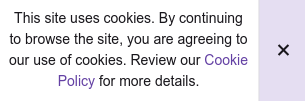
\includegraphics[width=0.6\linewidth]{sections/figures/cookie_usage_notification}
\caption[]{Cookie Usage Notification (English Version)}
\label{fig:cookie_usage_notification}
\end{figure}

In order to understand what information Twitch gathers on its users and how it is processed, we follow the given link to their Cookie Policy and analyze it. The entire Cookie Policy can be found in \cite{twitch-cookie-policy}. 

The main reason why Twitch uses trackers is to improve the users' online experience, as it states. Hereby, not only cookies, but also pixels and web beacons are listed as possible trackers (we explained these in~\sref{third-party-cookies}). Later in the policy though, all of these trackers are simply referred to as \textit{cookies}. For this reason, we assume that cookies are the type of tracker that enjoys the most prevalent usage by Twitch. 

The cookies are furthermore classified into \textit{Essential Cookies},\textit{ Performance Cookies}, \textit{Functionality Cookies}, \textit{Targeting or Advertising Cookies} as well as \textit{Flash Cookies}. Each type of cookie is responsible for a specific task. 

\subsubsection{Essential Cookies}\label{section:essential-cookies}
These cookies are, as stated, essential for the proper functioning of the website and the features it provides. One of these features is access to paid content. At this point, Twitch needs to know which privileges the user has already paid for and which not. This information is seemingly stored in form of a cookie on the user's PC. Another feature is restricted access to secured areas of the website. Without further information given, we assume that secured areas are the ones protected by authorization measures, like e.g. login necessity. The cookie used for this purpose is the one called \textit{twitch\_session\_id} (cf. ~\sref{technical-background}). This cookie is said to enable efficient navigation through the website. 

\subsubsection{Performance Cookies}
Technically, these are analytics cookies, such as \textit{Google Analytics} and \textit{Mixpanel}. The purpose of these cookies is to improve the way the site works. This is done by collecting information on which pages of the website are frequently used, whether any difficulties are being encountered, and whether the ads that are shown are clicked on by the users. 

\subsubsection{Functionality Cookies}
Functionality cookies can be used to customize website appearance to fit the preferences/settings of the current user. The Cookie Policy does not provide any examples for this type. From our experience though, the preferences mentioned could be the likes of chat color and preferred stream resolution. % Are these valid examples?

\subsubsection{Targeting or Advertising Cookies}
Targeting or Advertising Cookies provide ads that are more relevant to the user's interests. These cookies contain information on what the user has watched and which services provided by Twitch they have used. The platform allows itself to share this information with its partnered advertisement providers. A subsidiary of Google named \textit{DoubleClick} is mentioned. We assume that there might be a correlation between\textit{ Google Analytics} and \textit{DoubleClick}, as both services are technically powered by Google. Hence, internal information exchange between the two services seems likely. 

\subsubsection{Flash Cookies}
Flash Cookies are slightly different from the rest of cookies used, as we mentioned in the Technical Background~\sref{flash-cookies}. They cannot be deleted out of the user's browser, but instead have to be managed on the website of \textit{Adobe Flash Player}. Twitch uses this sort of cookies to deliver visual content to users, such as video clips and animations. Without Flash Cookies some of the streaming content provided by the platform is not available. 

\subsubsection{Third-Party Cookies}
The ``darkest'' part of Twitch's cookie world are Third-Party Cookies. These can be used by either extension developers for Twitch broadcasters, third-party advertisers, or ``other organizations'' \cite[Section~3]{twitch-cookie-policy}. 
\begin{itemize}
	\item \textit{Extension Developers} use cookies to allow user settings for these extensions. This set of cookies is limited to the extensions the user decided to opt in for. 
	\item \textit{Third-Party Advertisers} use cookies to collect information about the user's behavior on the websites of advertisements they might have clicked on. This way, the ads can be tailored with the  user's interests in mind. It is up to the advertisers to decide which way they do that. 
	\item We are not sure what Twitch means by the vague entity of \textit{``Other Organizations''}, because no further information on what these organizations are or what their cookies do is given. We only can guess that these organizations are not allowed to gather or use information beyond the limits of both the U.S. and local country's jurisdiction. For further inquiries, however, the email address \url{privacy@twitch.tv} is given. 
\end{itemize}

\subsubsection{Conclusion on Cookie Policy}
We conclude that Essential Cookies are the only ones that are necessarily needed for the website to function correctly. The rest of the cookies appear to be of only insignificant value to the user in terms of user experience. While the way Twitch treats data gathered by these cookies will be analyzed in the next section, we believe that the user may deactivate all but the Essential ones, without fearing significant service shortages. % Anything else?


\subsection{Privacy Policy} \label{section:privacy-policy}
Having analyzed the Cookie Policy, we switch our attention to the information given in the Privacy Policy of Twitch to determine the ways it treats its users' data. 

\subsubsection{What data Twitch gathers}
In their Privacy Policy, Twitch classifies the data being gathered into three different types:
\begin{enumerate}
	\item Information you can \textbf{provide to Twitch yourself} when using their services, such as:
	\begin{itemize}
		\item user name
		\item email address
		\item postal mailing address
		\item telephone number
		\item credit card number
		\item billing information
	\end{itemize} 
	\item Information Twitch \textbf{automatically collects} when you visit their website, such as: 
	\begin{itemize}
		\item IP address
		\item device type
		\item browser type
		\item software and system type
	\end{itemize}
	\item Information from \textbf{``other sources''}: In particular, if you have previously connected Twitch to one of their partners, which are mostly online social networks, Twitch can collect your data from these partners. However, it is not stated what kind of information this is. 
\end{enumerate} 

As we have previously seen, some of these data types are saved in cookies. Some other data might be stored directly on Twitch servers though, like e.g. your billing information. 

\subsubsection{What Twitch does with the data}
We already illuminated some of the things Twitch does with the data in the Cookie Policy section~\sref{cookie-policy}. The Privacy Policy extends the list of these data procedures in a significant way. 
 
For one, there is the feature to automatically install updates to the Twitch application on the user's computer. This procedure logically requires type 2 data (automatically collected data), such as device and operating system information. Without, it would not be possible to determine the correct update package. 

Another way Twitch uses our data is to communicate with the user, e.g. via email. Such reasons might be policy updates or promotional information. For the purpose of communication Twitch requires type 1 data (provided by users themselves), such as user name, email address, or postal address. 

Additionally, Twitch has to provide user information: 
\begin{itemize}
	\item in compliance with U.S. laws or user residence country laws
	\item in response to court order, judicial request or any other government request from the respective country~\footnote{The exact text of the policy might be better for accuracy purposes at this point: ``Twitch may disclose user information if we believe in good faith that such disclosure is necessary to comply with U.S. state and federal laws or other applicable laws around the world (for example, in the country of your residence), or respond to a court order, judicial or other government request, subpoena, or warrant in the manner legally required. '' \cite[Section~3]{twitch-privacy-policy}.}
\end{itemize}
Without proper legislative knowledge of the particular country, it is difficult to estimate the extent to which the platform is obligated to share user data with the governmental structures. In the light of recent government espionage scandals, it seems advisable to keep this in mind. 

Last but not least, Twitch retains the right to use data to protect itself from potential liability, third-party allegations and technically everything else that might damage Twitch as a company in any way. This point is vaguely formulated and leaves Twitch the necessary ``freedom of movement'' for the case of a force majeure situation. This part of the Privacy Policy makes us wary of the consequences for the user. It seems that in case of trouble, Twitch would not hesitate to put its own interests above the ones of the user. 

\subsubsection{Requirements to third-parties reusing the data}
There are some requirements that third-parties have to comply with if they want to reuse data that Twitch shared with them. The first one is to only use data for the purpose for which it was originally shared. Hence, if Twitch, for instance, shared a user's location with their partner Amazon for analytics purposes, the latter would not be allowed to reuse the data for marketing purposes. 

Another requirement to third-parties are potent confidentiality measures regarding the shared data. 

Twitch does not guarantee though that the partners' usage of data will comply with the Privacy Policy issued by Twitch. So technically, except for the two aforementioned points and the legal boundaries, the user does not know exactly what third parties do with their data. The only way to find this out is by working yourself through the Privacy Policies of these third-parties. However, Twitch states that it does not share information with third-parties that would allow them to personally identify its users. This means that the data Twitch shares with its partners is anonymous. 
Nevertheless, third-party advertisers can indirectly conclude on one's identity. If a user clicked on a certain ad that was meant to target a specific group of people, the ad provider could deduce the user's personality from it. 

\subsubsection{Data security}
Twitch does not by any means guarantee that the information users provide cannot be ``accessed, disclosed, altered, or destroyed by breach of any of [their] physical, technical, or managerial safeguards'' \cite[Section~10]{twitch-privacy-policy}. This way, Twitch makes sure that it cannot be held responsible for any type of technical failure. On the one hand, this sounds alarming, as it might seem that Twitch does not take data security seriously. On the other hand, Twitch is most likely aware of the effect that a massive data breach would have on its reputation. Hence, we assume that they do take the necessary measures to provide decent security of data. 

\subsubsection{Conclusion on Privacy Policy}
The conducted analysis of the Privacy Policy shows us that it is unlikely for Twitch itself to misuse its users' data. 
However, we could also see that the platform can both voluntarily (partners and ad providers) and involuntarily (governmental requests) disclose and share the users' data with other parties. While these third-parties underlie their own Privacy Policies and legislative regulations of their respective countries, it still cannot be concluded without doubt that the data they receive from Twitch will not be misused. 


\subsection{Data Flow}
Twitch's Cookie Policy and Privacy Policy gave us an insight into what types of data the company collects and how the data is being processed. To evaluate user information, Twitch essentially shares it with a number of entities (Fig.~\ref{fig:twitch_entities}). While working through the Privacy Policy issued by Twitch, we were not able to identify a paragraph which would mention that the platform's partners are not allowed to reshare the data they received from Twitch. This means that the travel of data originating from the user is in no way limited to the entities shown. Nevertheless, we hope that our excerpt from the data flow around Twitch is detailed enough to demonstrate the main dependencies of the big picture. 

% entities only
\begin{figure}[h!]
	\centering
	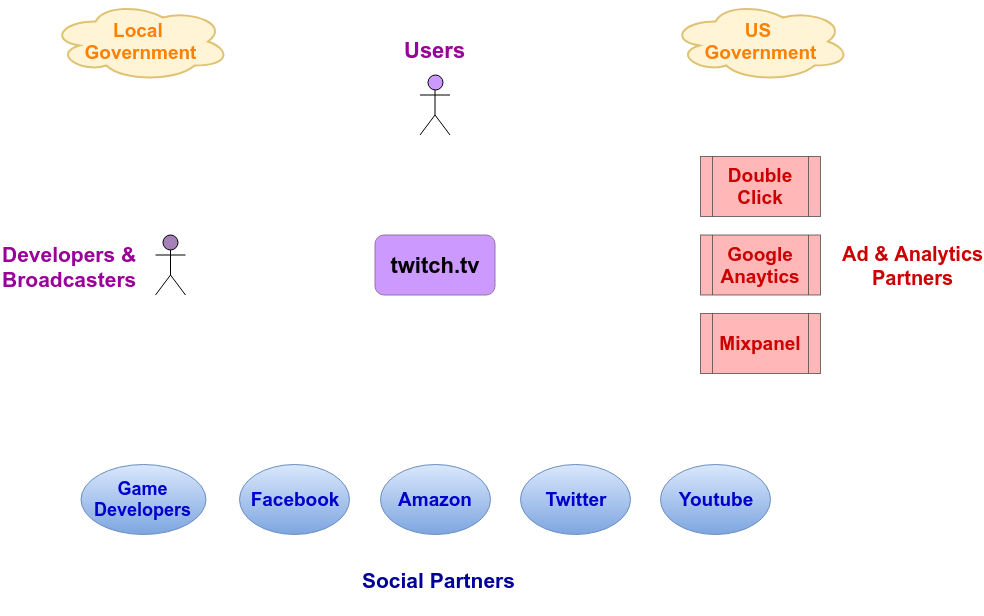
\includegraphics[width=0.9\linewidth]{sections/figures/twitch_entities}
	\caption{Entities involved in data flow with Twitch in the center}
	\label{fig:twitch_entities}
\end{figure}

On the one hand, there is the (simple) user of the services offered by Twitch. The user usually does not receive any personal data on other users or entities, and only serves as an origin to the information involved. In addition to that, the user sometimes fills the role of a 'trigger'. As soon as Twitch receives data from a newly registered user, it is able to request additional information on the person from both its \textit{Social} and \textit{Analytics Partners}. This process is significantly facilitated as soon as the user connected their Twitch account to one or more of the partners. This functionality is illustrated in Fig.\ref{fig:twitch_users}. 

% users - twitch
\begin{figure}[h!]
	\centering
	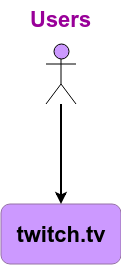
\includegraphics[height=0.3\linewidth]{sections/figures/twitch_users}
	\caption{Data flow between Twitch and its users}
	\label{fig:twitch_users}
\end{figure}

Keeping in mind that most of Twitch's relationships are bidirectional, the platform usually shares the newly acquired data on the registered user with its partners. The Privacy Policy does not directly state that Twitch is obligated to do so in exchange for information it receives from other entities. In the times of capitalism though, it seems likely that Twitch has to share its users' data the same way its partners do. This is especially the case for \textit{Social Partners}, as they do not receive monetary compensation for their services in contrast to \textit{Ad and Analytics Partners} like e.g. Google Analytics. A graphical visualization of Twitch's partner entities is shown in Fig.\ref{fig:twitch_partners}. To facilitate user information exchange with its partners, Twitch offers a feature in the user's profile settings called \textit{Recommended Connections}. On this page, the user can choose which social network, gaming console, or other partnered service they want to connect with their Twitch account. An example of the \textit{Recommended Connections} page is given in Fig.\ref{fig:recommended_connections} (appendix). 

% twitch - all partners
\begin{figure}[h!]
	\centering
	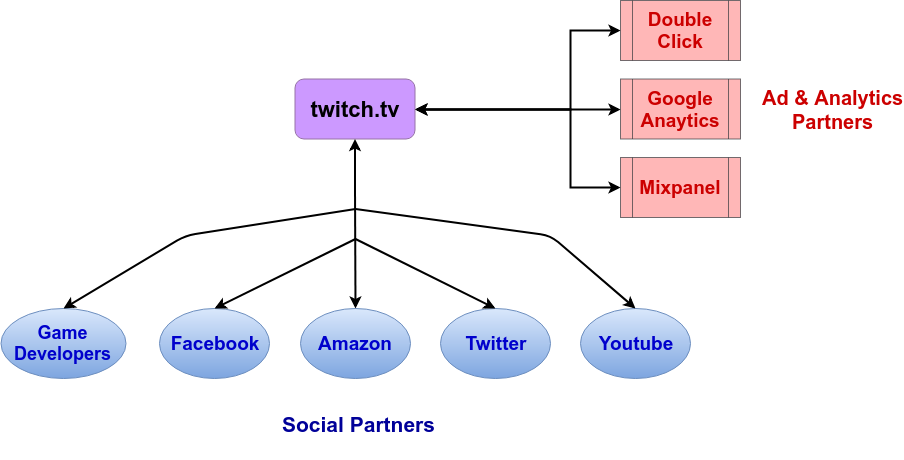
\includegraphics[width=0.9\linewidth]{sections/figures/twitch_partners}
	\caption{Data flow between Twitch and its social, advertisement and analytics partners}
	\label{fig:twitch_partners}
\end{figure}

Twitch partners and simple users are complemented by the ``advanced'' users. These are either \textit{broadcasters} or \textit{developers}. Broadcasters are the ones providing streaming content to Twitch users. Developers are the ones who either need to embed Twitch services in an external environment or to deliver various features and extensions to the broadcasters \footnote{The developers are frequently employees of gaming companies that want to embed Twitch streaming content into their gaming consoles/software. An example for such a console is the Blizzard Battle.net Desktop App: \cite{blizzard-desktop-app}.}. 

The main difference between simple users and advanced users lies in the amount of data they have to share with Twitch and the amount of data they receive from Twitch. While simple users are not obliged to share any personal data except for their user name and email address, they also have no access to other users' data. Developers and broadcasters, on the other hand, are obliged to share extended personal information such as their postal mail address and their billing details. In exchange for that, they do not only get advanced functionality of the platform, but they also gain access to information on other users. From a developer's point of view, the communication between developers and Twitch takes place over the so-called \textit{Twitch API} \cite{twitch-developers-platform, twitch-developers-guide}. The corresponding data flow is visualized in Fig.\ref{fig:twitch_broadcasters_developers}. 

% twitch - broadcasters and developers
\begin{figure}[h!]
	\centering
	
\includegraphics[width=0.6\linewidth]{sections/figures/twitch_broadcasters_developers}
	\caption{Data flow between Twitch, broadcasters and developers}
	\label{fig:twitch_broadcasters_developers}
\end{figure}

The last two major entities taking part in the data flow are the \textit{U.S. Government} and the \textit{Local Government} of the country where Twitch is being used (Fig.\ref{fig:twitch_government}). The reason why the U.S. Government is listed is because Twitch headquarters are based in San Francisco, California. 
The relationship between Twitch and these two \footnote{Or more, depending on how many countries are involved at once} entities is mostly unilateral. This is indicated by directed arrows from Twitch to the respective government in our graphic. The arrows are featured in a dotted notation, because Twitch does not view governmental structures as their direct partners. The possible data sharing with these entities is only listed in one of the paragraphs of Twitch's Privacy Policy. Hence, some of the platform's users might not directly be aware of the consequences of this relationship. The circumstances, under which user data might be shared with governmental structures we have previously covered in the Privacy Policy section. 

% twitch - government
\begin{figure}[h!]
	\centering
	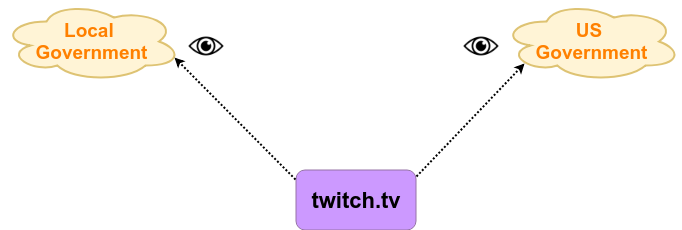
\includegraphics[width=0.7\linewidth]{sections/figures/twitch_government}
	\caption{Data flow between Twitch and governmental structures}
	\label{fig:twitch_government}
\end{figure}

We colored 'The Twitch Universe' accordingly to represent the data flow between the different entity classes. The full version of the data flow scheme can be seen in Fig.\ref{fig:twitch_data_universe}. 

In addition to the described data flow possibilities, Twitch states that in the event of a merger or sale, the entire user data saved on the platform's servers might need to be completely transferred to another company's storage servers. Such a procedure could result in major changes to the Privacy Policy. In this case, we recommend the user to timely take the policy changes into account, in order to make sure their data is treated as confidentially as before. 

% The entire Twitch Universe
\begin{figure}[h!]
	\centering
	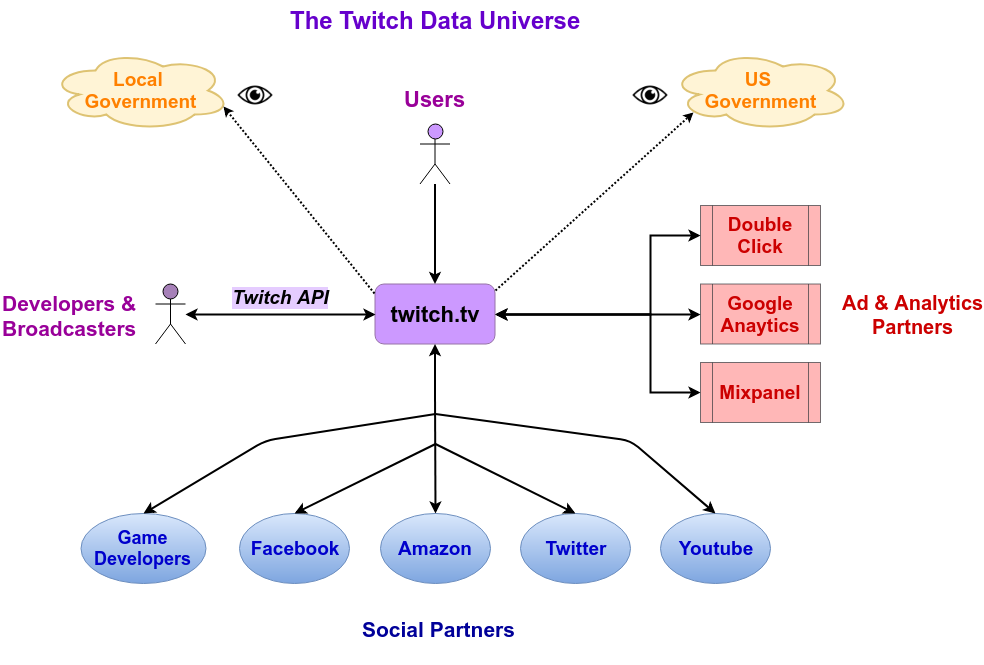
\includegraphics[width=0.9\linewidth]{sections/figures/twitch_data_universe}
	\caption{The Twitch Data Universe}
	\label{fig:twitch_data_universe}
\end{figure}

%Twitch to Partners: ''your username, the fact that your connection originated from the Twitch Services, and other relevant usage and diagnostic information), content you watch or your activities on the Twitch Services'' \\
%Twitch to Extension Developers: The same as in Automatically Collected Information only. 
%Twitch to Advertisers and Analytics Providers: The same as in Automatically Collected Information only. 

\subsection{Experimental Findings}
In order to determine the extent of tracking measures Twitch uses, we decided to conduct several experiments based on the information we were able to extract from its policies. 
We started with a 'clean' run to determine what sort of Twitch experience an ordinary user gets. For this purpose, we kept the allowance for all kinds of cookies to be placed on our experimental computer, switched off the VPN service, and took some other measures to make sure we behave like an ordinary user. 

Within this 'clean' run, the plugin Ghostery\footnote{Available under \cite{ghostery-plugin}}, which we preinstalled in our Google Chrome browser, indicated right away that there is a wide range of cookies used by the website. The particular cookies tracking us were: 
\begin{enumerate}
	\item Advertising Cookies
	\begin{itemize}
		\item Amazon Associates
		\item Datalogix
		\item ScoreCard Research Beacon
		\item Krux Digital
		\item Google Publisher Tags
		\item Google IMA
	\end{itemize}
	\item Analytics Cookies
	\begin{itemize}
		\item Google Analytics
		\item INFOnline
	\end{itemize}
\end{enumerate}
Interestingly, Ghostery did not list any Essential Cookies used on the homepage of \url{twitch.tv}, even though Twitch lists \textit{twitch\_session\_id} as one of the Essential Cookies they are using. 
Our first conclusion was that Ghostery might filter out the essential ones, while reducing the set of cookies shown to solely active trackers. To give ground to this assumption, we conducted the same experiment on other websites while using Ghostery. Our finding was that Ghostery, in fact, does show Essential Cookies after all, and even classifies them as such. 

Having found this out, we decided to check whether there are any cookies at all that are essential for Twitch to work properly. For this purpose, we went into our browser settings and checked the box to not allow any cookies and other trackers on our computer. After this, we once again tried visiting the homepage of Twitch. We instantly noticed that the page did not load at all. This leads us to the conclusion that Twitch does use Essential Cookies, just as the platform states itself in its Privacy and Cookie Policies. Hence, it seems that the plugin we used for determining the cookies does not always recognize the Essential Cookies for some reason. 
% check if it does without the other cookies and only with the essential ones

When looking into the list of cookies locally stored on our computer, we were able to find a wide range of cookies listed under the label \url{twitch.tv} in our browser's settings (Fig.\ref{fig:twitch-local-cookies}). 

% twitch - local cookies drop list
\begin{figure}[h!]
	\centering
	
\includegraphics[width=0.9\linewidth]{sections/figures/twitch_local_cookies}
	\caption{Section of our browser's cookie list with a drop list dedicated to twitch.tv}
	\label{fig:twitch-local-cookies}
\end{figure}

The number of cookies listed was 16. Our first guess was that some of these cookies could be outdated and derive from some previous Twitch usage on our experimental PC. We were proved wrong when we looked at the creation time stamp of each and every one of these cookies. All of the cookies seem to have been created within the time scope of our research, which consisted of several working units spread over one month. The cookies listed can be seen in Fig.\ref{fig:twitch-local-cookies-2} (appendix). 

At a closer look, most of the cookies proved to be structured similarly to the way we described it in the Technical Background~\sref{technical-background}. 
An example is given in Fig.\ref{fig:twitch-local-cookie-unique-id} (appendix). 

Another change in visual experience we noticed was that we got different advertisements shown when visiting a sample Twitch channel with cookies switched on and off. When cookie services were on, we had the ad by \url{pokerstars.de} played, whereas with cookies off we viewed an ad by \url{Epicenter.gg}. We were able to reproduce the outcome of this experiment by switching the 'incognito mode' on in our browser instead of disabling cookies. Apparently, the 'incognito mode' automatically switches off cookies and thus produces the same result. Besides the different advertisements, the streaming channel itself, which is shown on the homepage of \url{twitch.tv} on entrance did change as well, depending on whether we had cookies allowed or not. We were not able to identify a particular pattern though, as the welcoming streams were sometimes different and sometimes the same depending on the time of the day when we accessed Twitch. We assume that Twitch does use cookies to determine which stream should currently be shown to a particular user. It seems, however, likely that the algorithm behind this decision is complex and thus does not always produce a different result than if there were no cookies in use. 

While extending our experimental research on advertising, we noticed cases when our first visit on a Twitch streaming page caused an Amazon Prime advertisement to be shown, while any subsequent refreshing of the same page did not feature any ads at all. This might be a convenience feature, as Twitch users tend to refresh the page of the stream they are currently watching whenever the stream starts lagging or does not seem to load. When testing Twitch streams for an extended period of time, we noticed that such service behavior is quite frequent. The reason for this is that the Internet connection of each and single streamer may cause interruptions from time to time. This is especially the case in countries which do not provide solid Internet quality. 

In order to test whether Twitch optimizes the advertisements 'on the flow', we visited some of the commercial websites we thought Twitch might be partnered with to produce more income for the companies. Considering that Twitch is a streaming platform that is mostly used for video gaming content, the likes of \textit{MSI} and \textit{Razer} \footnote{\url{https://www.msi.com/index.php} and \url{https://www.razer.com/eu-en}, respectively.} seemed fitted for this experiment, as these companies produce some of the popular gaming hardware. Nevertheless, after visiting their respective websites and also some others, we did not notice any change in Twitch's advertisement policy in favor of either \textit{MSI} or \textit{Razer}. There are two possible explanations for that, namely: 
\begin{enumerate}
	\item Twitch is either not partnered with the specific companies we experimented with or simply not to an extent where it would optimize the user's ad experience in these companies' favor. 
	\item Twitch does optimize its advertisements in favor of such companies, but the algorithm is too slow on conclusions or too complex for any changes to take place within the timeframe of our experiment. This explanation seems likely in regard to modern machine learning algorithms, as their outcome is influenced by many different input parameters and not just by one or two, like visiting \textit{MSI} and \textit{Razer} webpages for instance. 
\end{enumerate}

Another case of cookie usage that we noticed, is that whenever we log in to the Twitch services with an account that is connected to \textit{Amazon Prime} services, we do not get any advertisements shown. This behavior is totally expected, considering that this is one of the widely advertised features of using both Amazon Prime and Twitch. Nevertheless, it is a valid example of how Twitch uses its Essential and Functionality cookies to improve user experience on its website. We mentioned gaining access to secured areas or features (like Amazon Prime features) of the website in the section on Essential Cookies~\sref{essential-cookies}. 

% TODO: Write an email to their privacy email address to check whether they seriously react to our privacy concerns 
%Twitch vows to respond to any such inquiry within 30 days of its receipt. //
%Suggestion: Californian law allows users to once a year request and receive a free-of-charge list of all third-parties who have obtained the user's data and what sort of data this exactly is. We could ask whether this only %applies to California or potentially to some other countries, specifically Germany, as well. 

%\subsection{Coverage in the media?}
%backup section in case we don't have enough

%\subsection{Things to keep in mind for how to avoid tracking section}
%Measures either advised or linked to by Twitch itself: 
%
%- Twitch provides the user with links which can be used to opt out of Targeting and Advertising Cookies by switching off some of the ad providers (links: youronlinechoices.com/uk/your-ad-choices or allaboutcookies.org/manage-cookies/index.html) \\
%- Guide on how to disable Flash Cookies \\
%- Third-party Cookies: =>  ''To disable or reject third-party cookies, please refer to the relevant third party’s website.'' \\
%- ''How do I control Cookies'' section is given at the end of the Cookie Policy webpage. \\
%- Twitch warns that if some of the cookies are disabled, it's services might not work properly. As we previously noticed in our experiments (ref.) section, it technically does not work at all in this case. (An ethical discussion might be useful at this place. ) \\
%- The user may decline to share ''certain information'' (ref. privacy policy) with Twitch \\
%- The user may disable their Twitch account (ref. privacy policy). Still, some of their information will remain stored on Twitch servers. \\
%- Opt out of Google Analytics: https://tools.google.com/dlpage/gaoptout \\
%- Opt out of Mixpanel: https://mixpanel.com/optout/ \\
%- Twitch does not respond to DNT (Do-Not-Track) services that some browsers provide, citing that ''the Internet industry is currently still working toward defining exactly what DNT means, what it means to comply with DNT, and a common approach to responding to DNT'' (ref. Privacy Policy - DNT Chapter)
%
%Also as mentioned in the conclusion to the cookie policy, one could simply deactivate the cookies that are not relevant to the performance with a plugin like Ghostery. 



